% TODO: 
% * Mention rdtsc() as replacement for a clock DONE
% * Update run and compile to return a success or failure value DONE
% * Clarify in case study: entropy parameter is only an illusrative artificial parameter to create randomness in measurements DONE
% * Update data format description in data.m UNREQUIRED

\section{Introduction}
Measuring and representing the performance of an algorithm represents quite a tedious task. Such activity requires a constant monitoring and intervention to collect data from an experiment, start the next one and check if everything works as expected. Such constant attention is error-prone. Once the data has been fully collected, it is often cumbersome and also error-prone to reshape it to a meaningful format such as a graph, or a format allowing the computation of such graph. There are many benefits in automatizing this process: making it autonomous, more reliable or faster.

The document introduces here a very simplified case study, where it is proposed to demonstrate the scalability of a multi-threaded program whose ``computation'' consists in achieving a given number of jumps through a loop. The sequential version takes the complete loop sequentially whereas the parallel implementation splits this loops in smaller chunks and distributes it equally among all threads. The performance of this program is monitored and plotted following a workflow and using tools introduced along the solving of this case study. The language used in this work is {C}, but any other programming language should work equally well. Also, the data is processed using Octave, but the scripts require little adaptation for Matlab. Section~\ref{sec:files} lists and briefly describes each files provided in the script set. Section~\ref{sec:problem} introduces the problem that illustrates this case study. Section~\ref{sec:process} details all the necessary steps to instrument a program, collect the results and use it to generate comprehensive representations. Finally, section~\ref{sec:conclusion} concludes the document.

%\section{Motivations}
%Measuring the performance of a computer program can be a very tedious task to do. Quite often, this involves the comparison of several different combinations of settings (such as the number of thread of memory allocate to the job) in order to observe how they affect the behavior of this program. Also, since many parameters can affect the performance to be measured, such as the underlying scheduler of the operating system, it is often a good practice to run each setting several times and extract statistical data rather to raw performance number. A high number of settings, combined with the necessity of running each program variants several times generates a high number of executions to supervise and makes it often difficult, if not impossible, to do it manually. An human operator can easily forget to change a parameter between two experiments, due to weariness or tiredness; as a consequence, the more an experiment contains settings to be manually changed, the higher is the risk of mistake at random steps of this experiments. In contrast, an automated process, when designed correctly, can repeat these tasks with no weariness nor tiredness and is much less subject to such errors.

%However, such automated process is difficult to design correctly. Possible reasons for these difficulties include bugs in the implementation of the automated process, but also a preference to automated experimental setup specifically targeted from their early development phases, to the observation of particular phenomenons the experiments aims to emphasize. Such strategy may shorten the development of the necessary scripting tools, but it has several drawbacks. It often results in the generation of semi human friendly data format, where data is shown in a semi-structural form surrounded by comments. Such formats are not easy to understand for humans, and require specific parsing tools to automatically gather fully structured data and generate visual representations of them. Because the tools are specifically developed for each experiments, outputs from different experiments are likely to have a different structure. This results in the necessity to rewrite the output parsers from one experiment to another and thus requires more efforts in the longer run. Moreover, because the data is collected aiming at the emphasize of a particular phenomenon, is is also often hard to reuse this data to show different properties. As a consequence it is necessary to design a new specific automated process, incompatible with other already existing tools because of too specific their characteristics. This results in even more necessary efforts to design and use an automated process in experimentation. Finally, a myriad of automated scripts quickly become cumbersome to use, because of their heterogeneous design resulting in heterogeneous user interfaces and workflows.

%Automated tools and a suitable workflow reduces these issues. It simplifies and unifies the process to automatically gather, structure and represent data collected through the performance measurements of as many program variants as the user and resources can afford to build and run automatically. here, the flow consists in several steps, from instrumentation of algorithm to data representation through data collection and processing. The method and tools are designed to be as general as possible, pushing specific steps as far as possible toward the instrumentation (early stage) and processing (late stage). In between these extreme, the data output from experiments take the same fully structured form of a numeric matrix, directly usable by scientific tools such as Matlab or its open-source competitor Octave. Such records are easily browsed through methods inspired from relational algebra and widely used in relational databases. This allows an easy extraction and transformation of interesting information, regardless of what the experiment specifically aimed at monitoring (provided that all necessary information was recorded). This information can be used to compute more simple matrices that can be directly represented in a visual form, using tools Matlab or Octave provide or more simple and complete handlers provided in the workflow and also described in this document.

\section{Requirements}
The user of the tools and workflow described in this document is expected to be acquainted with a number of technologies that are conjointly exploited in the flow. This includes basic knowledge of Bash, a confident use of Matlab or Octave scripting and notions in relational algebra or experience in databases\footnote{TDDD46 aims: Design and use a relational database, explain the theory behind the relational model and how this affects good design of databases.}. Debugging or developing the tools requires extensive knowledge in Bash and/or Matlab/Octave scripts. A sharp mastery of good programming practices is always most welcome. The reader can find introductory documentation on the internet about Bash~\cite{mikeg00,garrels08}, Make~\cite{anonymous_make_1,gnu_make}, Matlab scripts~\cite{huber97} and functions~\cite{recktenw95} (also applicable to Octave\footnote{http://www.gnu.org/software/octave/}), the C programming language~\cite{cprogramming} and Posix thread programming~\cite{tim10,barney12}.

\section{The set of scripts}
All the flow described in this document makes use of a set of scripts, composed of the files in the following list:
\begin{itemize}
\item start\\
Starts the compilation process or runs all experiments in one, unsupervised batch. Start it explicitly with bash (\emph{bash start ...}) instead of running it directly (incorrect: \emph{./start}). This file does not need to be modified under normal use, but only for contribution purpose. Refer to the sections \ref{sec:compile} and \ref{sec:run} more more information about it.
\item variables\\
Contains all the settings of the program and their possible values. Modify it for each different program or experiments. These values are read by \emph{start} (see above) when compiling or running program variants. See section~\ref{sec:plan} to get more information about this file. 
\item compile\\
Compile a variant of the program to be monitored. This script is called by \emph{start} and is given as parameters all settings defined as compilation settings as well as one value for each of them, in the same order as defined in the field ``compiled'' of the file \emph{variables}. Modify it to fit the program you want to monitor.
\item run\\
Runs a variant of the program to be monitored. It is called by \emph{start} with compile settings first then run settings and their associated value for one program variant, given as arguments.
\item settings\\
Various settings read by \emph{start} and that slightly affect its behavior. This files should not be modified nor even explicitly used.
\item merge\\
Merges the result of two experiments whose difference is not described in \emph{variables}. These two experiments must have output a result matrix having the same size and the same meaning for each of its columns. This script makes use of \emph{merge.m} and requires octave to work. Matlab cannot be used as an alternative.
\item data.m, data-xxxxx-yyyyyyy.m\\
Contains the raw values collected from all experiments and program variants \emph{start} compiled and ran. This file is automatically generated when \emph{bash start run <name>} finishes and should not be manually modified.
\item plot\_data.m\\
Experiment-specific Octave or Matlab script that reads the result output matrix produced by the program variants and \emph{start} when running them. This script transforms this data into smaller, ready to plot matrices. This file should be entirely re-written for all program to monitor. It can be expanded to extract other information from the raw output data.
\item octave/*.m, Matlab/*.m\\
Respectively Octave and Matlab specializations of data manipulation scripts, used by \emph{plot\_data.m}. Copy them into the same directory as the raw result file \emph{data.m} and run plot\_data.m from this directory (\emph{octave plot\_data.m} from the same directory, using Octave).
\end{itemize}

\section{The problem}
\label{sec:problem}
% Introduce the computation problem to be monitored and the way it has been paralellized
Suppose an algorithm that achieves some work in a sequential fashion, for instance the code shown in Fig.\ref{fig:do_some_work}. This sequential algorithm must be compared to an equivalent, parallel version. The parallelization of this algorithm is achieved through the division of $count$ by the number of threads employed, and every thread runs the loop with this new value of $count$. Since this example is very simple, the performance measurement reveal few differences from run to run. Not only this is usually not the case, but it alos prevent the illustration of the standard deviation plotting capability of this tool. Therefore $count$ variates more or less, randomeley, along another property named $entropy$, which models this missing performance randomness from run to run. The parallel implementation must show good scaling properties with the number of threads employed, and demonstrate an efficient use of them. This requires the computation load to be equally spread among the threads available; in other words, all threads must compute for a roughly equivalent period of time. Both global and per-thread computation time must be recorded and shown in a representation similar to Fig.\ref{fig:timing-200}. On this figure are represented the global computation time (red curve) as a function of number of threads, as well as individual threads' computation time for every situation, using the sequential algorithm or its parallel version using one to eight threads (the parallel version with one thread shows the overhead of parallelization). Both sequential and parallel implementations are available in appendices \ref{app:sequential} and \ref{app:parallel}, respectively. These implementations introduce 3 settings: the number of threads to use (degree of parallelism), the number of jumps the program must do (that models the size of the problem) and the entropy in performance described above. Each of these settings take their value from $\mathbb{N}$, $\mathbb{R}$ and $\left[0;1\right]$, respectively. Consequently, all variants of the algorithm are contained in a 3 dimensions space. Section~\ref{sec:process} explain the process to obtain a figure such as Fig.\ref{fig:timing-200}.

\begin{figure}
\centering
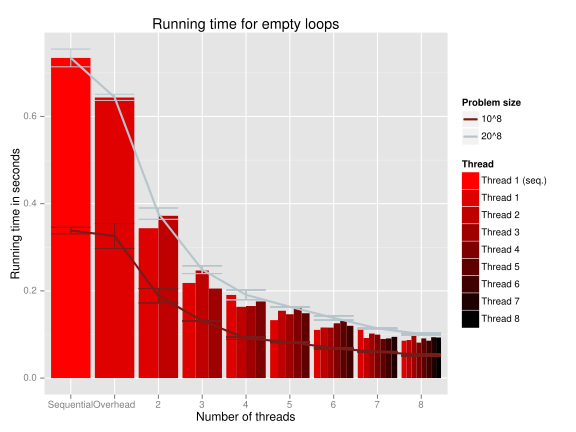
\includegraphics[width=10cm]{images/timing-200.eps}
\caption{Example of a plot obtained through the measure and plotting scripts set.}
\label{fig:timing-200}
\end{figure}

\begin{figure}
\centering
\begin{lstlisting}
static int
do_some_work(unsigned long long int count)
{
  unsigned long long int i;

  // Bring it on, yeah!
  for (i = 0; i < count; i++);

  return 0;
}
\end{lstlisting}
\caption{``Computation''-intensive algorithm used as case study in this tutorial.}
\label{fig:do_some_work}
\end{figure}

\section{Setting up an experiment, collecting, extracting and plotting data}
\label{sec:process}
Sections~\ref{sec:setup} through \ref{sec:format} describe all the necessary steps to take in order to safely monitor a program and generate a visual representation of the data gathered. All these steps take as case study the problem described in section~\ref{sec:problem}.

\subsection{Step 1: Set up your program}
\label{sec:setup}
%The effect of one or more settings on the general behavior and performance of an algorithm can be measured by measuring and comparing the performance of all variants defined by these settings. All differences between every variants not induced by these settings must be minimized as much as possible, so that only the differences these settings generate are measured. Considering an implementation of an algorithm always may need to be updated, keeping several copies of code with slight differences makes such maintenance difficult. At every necessary changes, the programmer has to update correctly every copies of the code and may forget one copy and/or commit a mistake while reporting the change in another copy. Such methodology may generate numerous copies to be maintained, which number grows exponentially with the number of settings and the number of value these settings can take. In addition, having one copy for each possible setting combinations makes difficult to obtain a new variant for which no additional copy of the code was dedicated.

%Instead of maintaining several copies for each setting to be tested, it is more advisable alter limited portions of a unique copy of the code, when compiling or running each variants. This can be done in two ways: either by giving the program an argument at runtime, either using preprocessor directives in the code that the compiler can interpret. Using preprocessor directives, the compiler can limit the compilation only to the relevant portions of code and using the right constant values, according to options given when compiling. This case studies illustrates argument passing to provide the size of the problem to be computed, as well as preprocessor directive to define both if the algorithm must be sequential or parallel (and in this case the number of threads to use) and the degree of entropy expected when measuring the performance.

Modify your source code to integrate several versions (sequential and parallel) to the same source file. A version or another is chosen through preprocessor directives (\#if, \#ifdef, \#ifndef, etc) at compilation time. Each directive takes a decision according to the value of definitions (defined by the directive \#define or passed by the compiler). A definition represents a \emph{setting} and takes one value among several possible. Use directives and definitions to select portions of codes that are specific to a program version, but keep these specific portions as small as possible. Figure~\ref{fig:directive} provides a simplified illustration of this technique; you can also find more example and information on the internet. Appendix~\ref{app:unified} shows the sequential and parallel version of the same algorithm merged into a single source file. Depending on the options given to the compiler (-D switch with gcc, see gcc --help), the sequential or a parallel version is compiled. The way the relevant options are given to the compiler is described in section~\ref{sec:compile}.

Another way to control the behavior of a program among different versions are arguments to the program when it is started. Depending on the values in argv, the program can branch to one or another portion of code. However, since this decision is taken at runtime, it can slow down the execution time of the program. This should be avoided if the execution time of the program is monitored.
%In {C}, such preprocessor directives are {\#if + condition over a constant symbol}, {\#ifdef + constant symbol} or its complement {\#ifndef + constant symbol}, respectively the following code if the condition is achieved when compiling the code, if the constant symbol is defined when compiling or if it is undefined at compilation time. The in Fig.\ref{fig:directive}, constant symbol is {NB\_THREADS}. All these preprocessor directives can be complemented using the {\#else} directive and must be ended by {\#endif} after the code which compilation is decided by this directive.

\begin{figure}
\centering
\begin{lstlisting}
#if NB_THREADS > 0
  pthread_t thread[NB_THREADS];
  pthread_attr_t attr;
  thread_do_some_work_arg arg[NB_THREADS];
  int i;

  pthread_attr_init(&attr);
  for (i = 0; i < NB_THREADS; i++)
    {
      arg[i].id = i;
      // influence the number of loops to
      // achieve by the value of entropy
      // to simulate performance randomness
      arg[i].count = variate(count, entropy);

      pthread_create(&thread[i], &attr,\
 thread_do_some_work, (void*) &arg[i]);
    }

  for (i = 0; i < NB_THREADS; i++)
    {
      pthread_join(thread[i], NULL);
    }
#else
  count = variate(count, entropy);
  do_some_work(count);
#endif
\end{lstlisting}
\caption{If the constant {NB\_THREAD} is defined to a value greater than zero when compiling this code, then a multi-threaded version of the code is compiled, using pthreads. Otherwise the sequential version is generated, that simply calls the function achieving the computation.}
\label{fig:directive}
\end{figure}

\subsection{Step 2: Monitor the performance}
\label{sec:instrument}
% The methodology can work with any measure relevant for the experiment, as long as it can be represented with a numeric value (either integer or float). Algorithms' performance can be measured through many dimensions, but a common metric is execution time. A {C} program can use functions such as $clock\_gettime()$ to measure the time with a precision up to the nanosecond. Refer to the documentation (man clock\_gettime) for more information. In this case study, $clock\_gettime()$ is used to measure the time when the algorithm or a thread starts and the time it stops. The difference between these two time stamps is the time the implementation took to run or a thread consumed to perform its task. $clock\_gettime()$ does not provide a unique number but two integers, denoting seconds and the second nanoseconds. Consequently, it is difficult to use this data in this format in the program code without a few calculations that can hinder the program's performance. Instead, this calculation is achieved in the processing phase (see section~\ref{sec:format}), where the performance do not alter the measurement. $clock\_gettime()$ gives the user the choice between five clocks, each having different properties. The following three clocks may be the most useful:
Record the values you want to measure into variables, and display these variables at the end of the program execution, or at a moment when outputting these values does not affect the values you want to measure. Collecting data generally affects execution speed. If you want to measure execution speed, remember that printf() is very slow and will affect the performance if it is used in the middle of the code you want to measure. Consider issues such as data locality and try to make as much profit of caches, but try not to take it all from the algorithm you monitor. This might significantly slow it down.

\subsection{Measure the time}
There are several functions provided by {C} and Linux to measure execution time. In general, a good resolution is better. clock\_gettime() allows the measurement of time with a precision of a nanosecond. The downside of this function is the format of this information, that takes shape in two integers, one counts seconds, the second nanoseconds. Such separate format makes difficult the fast calculation of interesting values. Later sections show that this can be done later in the process. Refer to man pages of clock\_gettime() to get more information about it (type ``man clock\_gettime'' in a Linux terminal). It can use several clocks, each of them having different properties. Below is a short description of three interesting clocks:

\begin{enumerate}
\item CLOCK\_THREAD\_CPUTIME\_ID\\
Computation time consumed by a thread. It does not take into account the time when the thread has been scheduled or blocked at a synchronization primitive. Consequently, it does not necessarily represent the time period between when the thread has been started and stopped. The use of this clock is safe to measure the thread execution time only when there is no synchronization involved in this thread and no more threads are used than the underlying computer has cores unused by any other thread in the system.
\item CLOCK\_PROCESS\_CPUTIME\_ID\\
Computation time consumed by the process. This is the time matching the sum of cycles consumed in parallel by all threads in the process. This time is not the time between the start and stop times of a process, equivalent to the execution time of its slowest thread. A process running two threads in parallel for 2 seconds is considered as having consumed 4 seconds of computation.
\item CLOCK\_MONOTONIC\\
System-wise clock, that is shared between every threads. CLOCK\_MONOTONIC provides a common time reference to every process or thread running in the system. This clock does not accumulate the computation time provided by parallel threads (as CLOCK\_PROCESS\_CPUTIME\_ID does), but it does not pause when a thread is scheduled or blocked (as CLOCK\_THREAD\_CPUTIME\_ID). It also count the time other programs running in the system consume. This is the preferred clock to measure time intervals if the computer is not already running an other computation-intensive program.
\end{enumerate}
%The choice of a correct clock is important to obtain the correct information when measuring performances. Appendix~\ref{app:clock} illustrates different results from running the same program compiled and run with the same parameters, except the choice of the clock used to monitor the performances. The reason why such difference arisen may not be obvious and can even interpreted as correct if not enough care is given to the correctness of the data collection method.

In order to calculate the time taken to execute a portion of code, $clock\_gettime()$ is called before and after each computation step being monitored. The difference between the two dates collected gives the execution time of the code between the first and the second collect of time. As described in section~\ref{sec:setup}, these instructions should be protected by preprocessor directives, making easy to recompile and run the program with no instrumentation instructions. Figure~\ref{fig:instrumentation} provides an example of such instrumentation and appendix~\ref{app:instrumented} provides a fully instrumented version of the {C} program.

\begin{figure}
\centering
\begin{lstlisting}
#ifdef MEASURE
  clock_gettime(CLOCK_MONOTONIC, &start);
#endif

  srandom(time(NULL));
  count = atoi(argv[1]);
  do_work(count, ENTROPY);

#ifdef MEASURE
  clock_gettime(CLOCK_MONOTONIC, &stop);

#if NB_THREADS > 0
  for (i = 0; i < NB_THREADS; i++)
    {
      printf("%i %i %li %i %li %i %li %i %li\n", i + 1,
          (int) start.tv_sec, start.tv_nsec, (int) stop.tv_sec,
          stop.tv_nsec, (int) thread_start[i].tv_sec,
          thread_start[i].tv_nsec, (int) thread_stop[i].tv_sec,
          thread_stop[i].tv_nsec);
    }
#else
  printf("%i %i %li %i %li %i %li %i %li\n", 0,
      (int)start.tv_sec, start.tv_nsec, (int)stop.tv_sec,
      stop.tv_nsec, (int)thread_start.tv_sec,
      thread_start.tv_nsec, (int)thread_stop.tv_sec,
      thread_stop.tv_nsec);
#endif
#endif

  // Always report a successful experiment
  return 0;
}
\end{lstlisting}
\caption{$clock\_gettime()$ before and after the portion of code being monitored collects the necessary data to compute the time used to run this portion of a program.}
\label{fig:instrumentation}
\end{figure}

\subsubsection{Choosing the right clock}
\label{app:clock}

In the figures~\ref{fig:monotonic} and \ref{fig:thread}, the same program has been compiled using the same settings, run on the same machine with the same input. Each variant has been run the same amount of time and the same script has been use to generate the plots. The only difference lies in the clock that has been used to measure the performance. The machine on which these two experiments have been run offers two cores. The difference in the measurement starts with the third core: in Fig.\ref{fig:monotonic}, the clock used to measure the execution time is global, and measures the real time. The clock used in Fig.\ref{fig:thread} considers the time as the number of processor clock ticks that was given to threads, not real time. As the machine only offers 2 cores, a third thread has to share its core with another thread, thus making CLOCK\_THREAD\_CPUTIME\_ID unsynchronized with real time. Notice one can use other processor or OS-provided functions to measure time. As an example, $rdtsc()$ takes profit of registers available on x86 archtectures from Pentium and returns on 64 bits the number of clock cycles elapsed since last processor reset. Figure~\ref{fig:rdtsc} shows an implementation taking profit of the relevant register in a function a regular C program can use.

\begin{figure}
\centering
\begin{lstlisting}
static void*
thread_do_some_work(void* arg)
{
  thread_do_some_work_arg *args;
  args = (thread_do_some_work_arg*) arg;

#ifdef MEASURE
  clock_gettime(CLOCK_MONOTONIC,\
 &thread_start[args->id]);
#endif

  do_some_work(args->count);

#ifdef MEASURE
  clock_gettime(CLOCK_MONOTONIC,\
 &thread_stop[args->id]);
#endif

  return NULL;
}
\end{lstlisting}
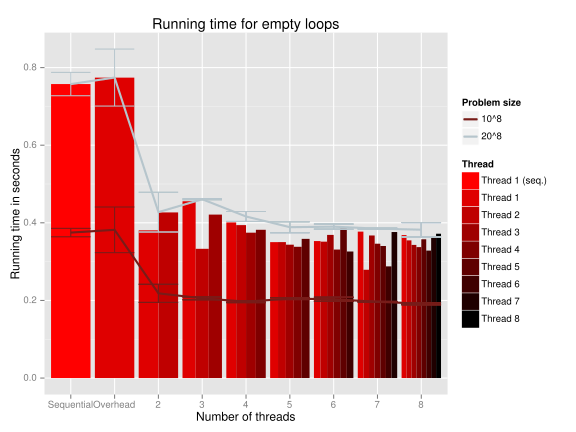
\includegraphics[width=10cm]{images/timing-200-nicolass-monotonic.eps}
%\label{fig:monotonic_graph}
%}
\caption{Code using CLOCK\_MONOTONIC to monitor time, and performance measured from the data collected.}
\label{fig:monotonic}
\end{figure}

\begin{figure}
\centering
\begin{lstlisting}
static void*
thread_do_some_work(void* arg)
{
  thread_do_some_work_arg *args;
  args = (thread_do_some_work_arg*) arg;

#ifdef MEASURE
  clock_gettime(CLOCK_THREAD_CPUTIME_ID,\
 &thread_start[args->id]);
#endif

  do_some_work(args->count);

#ifdef MEASURE
  clock_gettime(CLOCK_THREAD_CPUTIME_ID,\
 &thread_stop[args->id]);
#endif

  return NULL;
}
\end{lstlisting}
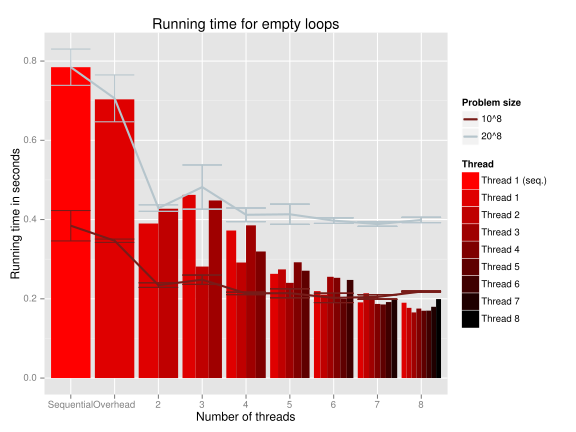
\includegraphics[width=10cm]{images/timing-200-nicolass-thread.eps}
\caption{Code using CLOCK\_THREAD\_CPUTIME\_ID to monitor time, and performance measured from the data collected.}
\label{fig:thread}
\end{figure}

\begin{figure}
\centering
\begin{lstlisting}
#ifdef __i386
extern __inline__ uint64_t rdtsc() {
  uint64_t x;
  __asm__ volatile ("rdtsc" : "=A" (x));
  return x;
}
#elif defined __amd64
extern __inline__ uint64_t rdtsc() {
  uint64_t a, d;
  __asm__ volatile ("rdtsc" : "=a" (a), "=d" (d));
  return (d<<32) | a;
}
#endif
\end{lstlisting}
\caption{C inline assembly implementation of rdtsc using hardware registers.}
\label{fig:rdtsc}
\end{figure}

\subsubsection{Output the data collected}

The program whose performance is monitored must report the data in a specific way, that allows the expression of any numeric data measured. This data must take the shape of a matrix, which is represented by its values separated by a space, as shown in figure~\ref{fig:output}. In this matrix, each column represents a value of a feature measured, or information related to that value (such as the thread id corresponding to a thread's execution time). A line represents a feature's instance (one line per thread). This is the case in this example.

Figure~\ref{fig:output} shows the output of the instrumented program of this case study. The first column represents the thread number (there are 8 threads used in this experiment), the second column is the time in seconds when the algorithm was started and the third is the time in nanoseconds (added to the seconds of the second column) when the program was started. The next two columns represent in the same format the time when the program stopped. The four next values represent the start and stop time for every thread. 

Notice that the four columns from 2 to 5 are identical in every line, as this information is global to the program and not thread-specific. Columns 6 to 9 are different in each line, since each of them show the execution time of one thread. The reason why global data is repeated is because the format of a matrix \emph{must} be preserved, in order to be parsed in further steps. In addition, all values must be numeric, integer or decimal.

\begin{figure}
\centering
\begin{lstlisting}
1 28689 94... 28690 27... 28689 942207530 28690 270489437
2 28689 94... 28690 27... 28689 942220041 28690 250966917
3 28689 94... 28690 27... 28689 948509233 28690 254110653
4 28689 94... 28690 27... 28689 948318059 28690 269370024
5 28689 94... 28690 27... 28689 948004682 28690 270454439
6 28689 94... 28690 27... 28689 943606755 28690 264533334
7 28689 94... 28690 27... 28689 942284021 28690 265217907
8 28689 94... 28690 27... 28689 956254814 28690 268802904
\end{lstlisting}
\caption{Format the data must take when output from an instrumented program.}
\label{fig:output}
\end{figure}

Once data is produced or in case of any failure, it is important to exit the program with a relevant exit value (\emph{return 0}). Returning 0 reports a run to work as expected and output to be taken into account. A return value different than 0 denotes a unsuccessful run and will make the batch to discard output produced. See section~\ref{sec:run} for more details about return values and the way they are handled.

%The collected data must be forwarded to the scripts managing the experiment through I/O:s, usually by writing them on the screen or to a file. Such operation must be performed with caution, as I/O:s are very slow and may affect the performance measurement. This can happen when some threads output the data they collected when the global performance are still measured. Instead of writing these results through an I/O, it is more advisable to store them in memory and output them at the end of the program execution, when all timing measurements are finished and performance penalties are not important anymore, as shown in Fig.~\ref{fig:instrumentation}. However, read and write operations to main memory can also be slow and hinder the performance when measuring them. This effect can be minimized by using much faster memories such as caches, but such memories are also typically small, shared with the algorithm being measured and required by this algorithm to perform faster. Select carefully the data to be collected in order to reduce the necessary memory to store them and reduce the impact on the algorithm's performance. There is no solution to eliminate all influence on performance when collecting data, but this effect can and should be lowered at most.
% Collect start and stop time, using clock_gettime with its different clocks
% Avoid printf nor I/O in the middle of your experiments, as this is very slow and can artifically reduce the performance measured
% Instead, collect numbers and store them in memory
% Do not store too much data as main memory can also be slow and reduce the performance; consider cache-miss issues
% Select carefully the data you want to measure.

\subsection{Step 3: Set up the different compilation and runtime settings to be used}
\label{sec:plan}
The scripts use the content of the file \emph{variables} to build the complete list of possible versions the program can have, and that must be compiled. This list of versions is also used to run and collect data from all possible versions. The settings' names and the values they can take are written using the syntax for Bash scripts. As discussed in section~\ref{sec:setup}, settings' values can be given as programs' runtime arguments or preprocessor directives resolved at compilation time. This distinction must be made when filling settings' names and possible values in \emph{variables}. Appendix~\ref{app:variables} gives a complete example of this file. Several variables need to be filled:
\begin{itemize}
\item output\\
Describes the meaning of each column of the matrix the program outputs when sending the data it measured (one word per column). Elements are separated by a space and the list must be surrounded by double quotes(").
\item compile\\
List of the settings whose value is given at compilation time to the {C} preprocessor. All elements are separated by a space and the list is surrounded by \emph{parentheses} only (no double quotes). Elements of this list cannot take some name such as \emph{count}, as these names are used in other parts of the scripts and their use can randomly alter the good functioning of the scripts. There is no exhaustive list of these forbidden values, so users are encouraged to report them.
\item run\\
List of the settings whose value is given at runtime to the program as an argument. This field has the same limitations and constraints as \emph{compile}. The names used in \emph{compile} and \emph{run} are mutually exclusive.
\end{itemize}
Every element in \emph{run} and \emph{compile} lists must be defined as a variable, taking as values the list of all possible value this setting can take. This list must be surrounded by double quotes.

\subsection{Step 4: Compile your program}
\label{sec:compile}
It is a good practice to provide a Makefile to build your program. The syntax of a Makefile is not described in this document. Refer to make's manual\footnote{http://www.gnu.org/s/make/} for this, or browse the internet for examples. Section~\ref{app:makefile} gives the one used in this case study and Fig.\ref{fig:makefile} shows the important lines in the context of this section. What is important to know here is that make and Makefiles can take arguments of the form $argument=value$ when invoking the make tool. This argument is interpreted as a variable taking this value in the Makefile. Figure~\ref{fig:makefile} shows that gcc is called in order to compile program.c to a binary output whose name depends on a suffix given when make is invoked. GCC also takes as arguments {CFLAGS}, that defines the constant symbols {MEASURE}, {NB\_THREADS} and {ENTROPY}. The two latter symbols take respectively the value of the makefile's variables {NB\_THREADS} and {ENTROPY}, which are given as arguments when invoking make. {CFLAGS} also includes switches such as {-Wall} that forces a more strict control on the code and {-O0} which disables every optimizations the compiler could provide. The former flag is a good programming practice while the latter is important to make sure that no unexpected optimization can alter the behavior of the code, thus allowing more accurate performance measurements. {-g} and other flags enable debugging and provide with the linker the libraries that the program has to be linked with.

\begin{figure}
\centering
\begin{lstlisting}
CFLAGS=-g -O0 -Wall -lrt -pthread -DMEASURE\t
 -DNB_THREADS=$(NB_THREADS) -DENTROPY=$(ENTROPY)
[...]
	gcc $(CFLAGS) -o program$(SUFFIX) program.c
\end{lstlisting}
\caption{GCC is invoked with options defining symbols handled by the {C} preprocessor directives (\#if, etc).}
\label{fig:makefile}
\end{figure}

More focus in this case study is given to the file \emph{compile}, as this file is called once per variant to be compiled with the list of compilation settings and one possible combination given as arguments. A complete version of this file written in Bash is given in appendix\ref{app:compile} and its most important parts are illustrated in Fig.\ref{fig:compile}. The arguments are given in the same order as the list described in section~\ref{sec:plan}. In this case study, \$1 defines the entropy and in \$2 is given the number of threads that have to be compiled in this version. It is a good practice to assign these values to variables whose name is comprehensive. This clarifies what information is used in every line of the script, and facilitates the propagation of changes from \emph{variables} to \emph{compile}. Figure~\ref{fig:compile} shows that make is called with arguments defining {ENTROPY} to the value of the entropy setting for this compilation as well as the number of threads to use. At the binary output's file name is appended the value of entropy and number of threads. Having a separate name for each compiled program variants prevents variant from being overwritten by each other, and makes it possible to start the right version when a particular measurement is to be started. Notice \emph{compile} must return a value so the global batch knows if it succeed or not. This is achieved with \emph{exit <value>} where \emph{<value>} is the value to return. 0 denote success and anything else report a failure. A convenient way to obtain a suitable value consists in reading \emph{\$?}, which returns same value as the last program or command called, usually having the same convention.

\begin{figure}
\centering
\begin{lstlisting}
entropy=$1
nb_threads=$2

make ENTROPY=$entropy NB_THREADS=$nb_threads\
 SUFFIX=-$entropy-$nb_threads
\end{lstlisting}
\caption{\emph{compile} catches the values of compilations settings and passes them to make.}
\label{fig:compile}
\end{figure}

Once the files \emph{variables} and \emph{compile} are ready, the compilation process is started with the command \emph{bash start compile}.

\subsection{Step 5: Run your experiments}
\label{sec:run}
All algorithm's variants are run through the bash script \emph{run}, that, similarly to \emph{compile} (see section~\ref{sec:compile}) takes as arguments one possible combination of all the settings each time it is called. An example of this file is given in appendix~\ref{app:run} and illustrated in Fig.~\ref{fig:run}. The compilation settings are given first then the runtime settings are appended, both taken from \emph{variables}. In this example, arguments 1 through 2 are taken from the compilation settings and arguments 3 and 4 represent the runtime settings. The binary file whose file name has for suffix the matching entropy value and number of threads is executed with the runtime argument ct, that defines the number of jumps the program has to perform. The parameter \emph{try} is never used and stands only to run several times (defined in \emph{variables} as 1 to 10) the same variant.

\begin{figure}
\centering
\begin{lstlisting}
#!/bin/bash -f

# compilation settings
entropy=$1
nb_threads=$2

# run settings
ct=$3
try=$4

./program-$entropy-$nb_threads $ct

exit ?
\end{lstlisting}
\caption{\emph{run} catches the compilation settings first, then the run settings and run the right binary with relevant parameters.}
\label{fig:run}
\end{figure}

In order to make the scripts catch their output from the measurements, \emph{run} must absolutely print on standard output the matrix generated by the program variant, regardless of the way it outputs the data collected. \emph{run} must output this matrix, and nothing else, to standard output. On this example, the program variant directly prints it on the terminal. It may also display data files the program would generate, after some possible filtering. As for \emph{compile} script (see section~\ref{sec:compil}), it is very important the \emph{run} script returns 0 if the experiment was successful or another value in case of failure. The use the keyword \emph{exist} and special variable \emph{\$?} is suitable to this purpose.

% Very rough time estimation algorithm
% Give a name to your experiment; if you run it again with more settings but the same code, the data will be merged together
Once the file \emph{variables} is ready and the compilation process is finished, all program variants are run and by the command \emph{bash start run $<name>$}, where $<name>$ is a name to the experiment being conducted. The script catches the data outputted on standard output, and stores it into the file \emph{data-$<name>$-$<date>$.m}. The batch script tries to give a very rough estimation of the remaining time before the batch is finished. This evaluation is based on the time that was necessary to run the program versions already run and is calculated using integer seconds only. It is therefore very rough and shouldn't be used to estimate the perfomance of the program monitored. If a variant run did not work properly and \emph{run} reported this failure through exit value, then the batch will record its output and neutralize it through comments and warnings in the final data file. As a consequence, failures do not necessarily jeopardize the whole measurement process, since their output are identified, neutralized. The faulty variant can be fixed and run in a later batch using the same experiment name. Alternatively, since incorrect output is not entirely discarded but only commented, the user can still collect it manually and analyze it if necessary.

If two experiments are successively run with the same name, their results are merged together into a single file named \emph{data.m}. Every experiment runs separately stores its result in a specific output file. The results of two experiments of the same name can be merged again to \emph{data.m} using the command \emph{bash start merge $<name>$}. Two different experiments, that differ in features that are not defined by any setting in \emph{variables} can be merged together by the command \emph{bash merge $<res1.m>$ $<res2.m>$}, to a file name \emph{MERGE-} followed by the two file names. In this file, data coming from one or another experiment can be identified thanks to an additional column inserted before the first column or original data. It takes as value the index of the arguments given to \emph{merge} that referred to its original result file, starting at 0. For instance, in the output of \emph{merge exp1.m exp2.m}, all data found in exp1.m will be prefixed by 0 and all data coming from exp2.m is prefixed by 1 in the output merged file. Note that this feature requires Octave installed, and that Matlab does not support such operation.

\subsection{Step 6: Process and plot the data collected}
\label{sec:format}
The data generated when running all program variants associates in a cell a numeric matrix and descriptive names for each columns of the matrix. Matlab or Octave can load directly this generated data and manipulate it. In order to ease the manipulation, several functions inspired from relational algebra are provided and data fields are addressable through their names. A complete commented example for this case study is available in the file \emph{plot\_data.m}. This script run by Matlab or Octave collects the data and processes it to obtain specific results used to plot graphs. It relies mainly on a set of data manipulation routines shortly described below. This script is usually very dense regarding the meaning of its lines, which makes it difficult to write correctly or to find the source of its defects. It usually takes shape of three parts: the first part collects the data, filters it through \emph{select} and \emph{where} operations and transforms it by applying custom functions. In this example such functions take recorded start and stop times (global and per thread) through their values in seconds and nanoseconds and compute the time in millisecond between these two steps in the program run. The second part extracts and reshapes this data in order to obtain small matrices ready to be plot. Finally, the third part uses the plot functions to generate and format graphs, and stores them in graphic files.

Below is a very short description of the functions available. More extensive documentation is available in the files where these functions are implemented:
\begin{itemize}
\item select\\
Filters the input matrix and keeps only the columns whose indexes are given as parameters (select.m).
\item duplicate\\ 
Duplicates once or more one or several columns of the input matrix.
\item where\\
Select matrices' row that fulfills conjunctive and/or disjunctive conditions (where.m)
\item apply\\
Applies a custom function and writes its result to the columns which index is given in arguments (apply.m).
\item groupby\\
Separates and groups rows by the content of the columns whose index is given as argument (groupby.m)
\item reduce\\
Reduces groups produced by groupby to one row per group, using reduction functions such as mean, standard deviation or custom functions. Merges rows to a matrix (reduce.m)
\item extend\\
Makes sure every groups has the same number of rows and inserts new rows with suitable data if necessary (extend.m)
\item cellfindstr\\
Finds and return the index of a string in a cell of strings. Returns 0 if the string could not be found
\item coln\\
Returns all column names of a table
\item data\\
Returns data matrix contained in the table
\item insert\\
Inserts and add a matrix into a table
\item setc\\
Replaces all column names in a table with names given as argument
\item setd\\
Replaces data matrix in table with data given as argument
\end{itemize}

Matrices can be plotted using the following plotting routines:
\begin{itemize}
\item quickplot\\
Plots one or more curves into a graph and displays axis labels, curves legend and graph title in a flexible way (quickplot.m)
\item quickerrorbar\\
Same as quickplot, but also allows the plotting of error bars (quickerrorbar.m)
\item quickbar\\
Plots a histograms with one or more bars per element in the x axis (quickbar.m)
\item quickgantt\\
Draws a gantt diagram, one horizontal line per element (quickgantt.m)
\end{itemize}

The command \emph{octave plot\_data.m} runs the octave script named \emph{plot\_data.m} and generates the graphs. Matlab cannot run the script in the same way. Open Matlab and browse in the left frame until you reach the folder where the results and all the scripts are stored, then start the script ``plot\_data.m''. The example used as a case study in this document produces the graph shown in Fig.\ref{fig:timing-200}. Its shows the time to perform 200 millions jumps using a sequential loop or splitting it between 1 to 8 threads. The plots clearly show that the global time decreases with the number of threads and it shows that the computation load is distributed equally among the threads. Finally, the low difference between the sequential and the parallel version using one thread shows that the overhead of parallelization is negligible compared to the overall performance.

\section{Conclusion}
\label{sec:conclusion}
This documents describes a general methodology to manage easily the run of several variants of a single algorithm implementation, and the collection, processing and representation of collected data. This is a tedious task that the tools described here make both easier and faster. Although they considerably reduce the occasions to commit mistakes in experiments due to human interventions, they do not eliminate such mistake. One possible remaining pitfall lies in the data collection method (the choice of the clock) and the parts that could not be automated. A too big confidence in this automated process may hinder cautions to take when performing the remaining manual interventions, or even simply makes the user to forget these steps even if they may be important. More efforts need to be done to improve the set of scripts described here, such as providing them with the ability to interrupt and resume an experiment. Contributions are encouraged, both through coding more functionality or bug reports.

\clearpage
\appendix
\section{Program to monitor performance}
\label{sec:files}
\subsection{Sequential version}
\label{app:sequential}
\begin{lstlisting}
#include <stdio.h>
#include <time.h>
#include <stdio.h>
#include <stdlib.h>
#include <pthread.h>

/* to be defined at compile-time:
 * ENTROPY
 */

static int
do_some_work(unsigned long long int count)
{
  unsigned long long int i;

  // Bring it on, yeah!
  for (i = 0; i < count; i++)
    ;

  return 0;
}

static unsigned long long int
variate(unsigned long long int count, float entropy)
{
  unsigned long long int variation, res;
  variation = (unsigned long long int) ((((float) (random() % RAND_MAX))
 / RAND_MAX) * count
      * entropy);

  res = (unsigned long long int) (((float) (count + variation))
 / (NB_THREADS
      == 0 ? 1 : NB_THREADS));

  return res;
}

static int
do_work(unsigned long long int count, float entropy)
{
  count = variate(count, entropy);
  do_some_work(count);

  return 0;
}

int
main(int argc, char ** argv)
{
  unsigned long long int count;

  srandom(time(NULL));
  count = atoi(argv[1]);
  do_work(count, ENTROPY);

  return 0;
}
\end{lstlisting}
\subsection{Multithreaded version}
\label{app:parallel}
\begin{lstlisting}
#include <stdio.h>
#include <time.h>
#include <stdio.h>
#include <stdlib.h>
#include <pthread.h>

/* to be defined at compile-time:
 * NB_THREADS
 * ENTROPY
 */

typedef struct
{
  int id;
  unsigned long long int count;
} thread_do_some_work_arg;

static int
do_some_work(unsigned long long int count)
{
  unsigned long long int i;

  // Bring it on, yeah!
  for (i = 0; i < count; i++)
    ;

  return 0;
}

static void*
thread_do_some_work(void* arg)
{
  thread_do_some_work_arg *args;
  args = (thread_do_some_work_arg*) arg;

  do_some_work(args->count);

  return NULL;
}

static unsigned long long int
variate(unsigned long long int count, float entropy)
{
  unsigned long long int variation, res;
  variation = (unsigned long long int) ((((float) (random()
 % RAND_MAX)) / RAND_MAX) * count
      * entropy);

  res = (unsigned long long int) (((float) (count +
 variation)) / (NB_THREADS
      == 0 ? 1 : NB_THREADS));

  return res;
}

static int
do_work(unsigned long long int count, float entropy)
{
  pthread_t thread[NB_THREADS];
  pthread_attr_t attr;
  thread_do_some_work_arg arg[NB_THREADS];
  int i;

  pthread_attr_init(&attr);
  for (i = 0; i < NB_THREADS; i++)
    {
      arg[i].id = i;
      arg[i].count = variate(count, entropy);

      pthread_create(&thread[i], &attr,
thread_do_some_work, (void*) &arg[i]);
    }

  for (i = 0; i < NB_THREADS; i++)
    {
      pthread_join(thread[i], NULL);
    }

  return 0;
}

int
main(int argc, char ** argv)
{
  unsigned long long int count;

  srandom(time(NULL));
  count = atoi(argv[1]);
  do_work(count, ENTROPY);

  return 0;
}
\end{lstlisting}
\subsection{Unified sequential and multithreaded versions}
\label{app:unified}
\begin{lstlisting}
#include <stdio.h>
#include <time.h>
#include <stdio.h>
#include <stdlib.h>
#include <pthread.h>

/* to be defined at compile-time:
 * NB_THREADS
 * ENTROPY
 */

#if NB_THREADS > 0
typedef struct
{
  int id;
  unsigned long long int count;
} thread_do_some_work_arg;
#endif

static int
do_some_work(unsigned long long int count)
{
  unsigned long long int i;

  // Bring it on, yeah!
  for (i = 0; i < count; i++)
    ;

  return 0;
}

#if NB_THREADS > 0
static void*
thread_do_some_work(void* arg)
{
  thread_do_some_work_arg *args;
  args = (thread_do_some_work_arg*) arg;

  do_some_work(args->count);

  return NULL;
}
#endif

static unsigned long long int
variate(unsigned long long int count, float entropy)
{
  unsigned long long int variation, res;
  variation = (unsigned long long int) ((((float) (random()
 % RAND_MAX)) / RAND_MAX) * count
      * entropy);

  res = (unsigned long long int) (((float) (count +
 variation)) / (NB_THREADS
      == 0 ? 1 : NB_THREADS));

  return res;
}

static int
do_work(unsigned long long int count, float entropy)
{
#if NB_THREADS > 0
  pthread_t thread[NB_THREADS];
  pthread_attr_t attr;
  thread_do_some_work_arg arg[NB_THREADS];
  int i;

  pthread_attr_init(&attr);
  for (i = 0; i < NB_THREADS; i++)
    {
      arg[i].id = i;
      arg[i].count = variate(count, entropy);

      pthread_create(&thread[i], &attr,
 thread_do_some_work, (void*) &arg[i]);
    }

  for (i = 0; i < NB_THREADS; i++)
    {
      pthread_join(thread[i], NULL);
    }
#else
  count = variate(count, entropy);
  do_some_work(count);

#endif
  return 0;
}

int
main(int argc, char ** argv)
{
  unsigned long long int count;

  srandom(time(NULL));
  count = atoi(argv[1]);
  do_work(count, ENTROPY);

  return 0;
}
\end{lstlisting}

\section{Fully instrumented C program}
\label{app:instrumented}
\begin{lstlisting}
#include <stdio.h>
#include <time.h>
#include <stdio.h>
#include <stdlib.h>
#include <pthread.h>

/* to be defined at compile-time:
 * NB_THREADS
 * ENTROPY
 */

#if NB_THREADS > 0
typedef struct
{
  int id;
  unsigned long long int count;
} thread_do_some_work_arg;
#endif

#ifdef MEASURE
#if NB_THREADS > 0
struct timespec thread_start[NB_THREADS],
 thread_stop[NB_THREADS];
#else
struct timespec thread_start, thread_stop;
#endif
#endif

static int
do_some_work(unsigned long long int count)
{
  unsigned long long int i;

  // Bring it on, yeah!
  for (i = 0; i < count; i++)
    ;

  return 0;
}

#if NB_THREADS > 0
static void*
thread_do_some_work(void* arg)
{
  thread_do_some_work_arg *args;
  args = (thread_do_some_work_arg*) arg;

#ifdef MEASURE
  clock_gettime(CLOCK_MONOTONIC, &thread_start[args->id]);
#endif

  do_some_work(args->count);

#ifdef MEASURE
  clock_gettime(CLOCK_MONOTONIC, &thread_stop[args->id]);
#endif

  return NULL;
}
#endif

static unsigned long long int
variate(unsigned long long int count, float entropy)
{
  unsigned long long int variation, res;
  variation = (unsigned long long int) ((((float) (random()
 % RAND_MAX)) / RAND_MAX) * count
      * entropy);

  res = (unsigned long long int) (((float) (count +
 variation)) / (NB_THREADS
      == 0 ? 1 : NB_THREADS));

  return res;
}

static int
do_work(unsigned long long int count, float entropy)
{
#if NB_THREADS > 0
  pthread_t thread[NB_THREADS];
  pthread_attr_t attr;
  thread_do_some_work_arg arg[NB_THREADS];
  int i;

  pthread_attr_init(&attr);
  for (i = 0; i < NB_THREADS; i++)
    {
      arg[i].id = i;
      arg[i].count = variate(count, entropy);

      pthread_create(&thread[i], &attr, thread_do_some_work,
 (void*) &arg[i]);
    }

  for (i = 0; i < NB_THREADS; i++)
    {
      pthread_join(thread[i], NULL);
    }
#else

#ifdef MEASURE
  clock_gettime(CLOCK_MONOTONIC, &thread_start);
#endif

  count = variate(count, entropy);
  do_some_work(count);

#ifdef MEASURE
  clock_gettime(CLOCK_MONOTONIC, &thread_stop);
#endif

#endif
  return 0;
}

int
main(int argc, char ** argv)
{
  unsigned long long int count;
#ifdef MEASURE
#if NB_THREADS > 0
  int i;
#endif
  struct timespec start, stop;
#endif

#ifdef MEASURE
  clock_gettime(CLOCK_MONOTONIC, &start);
#endif

  srandom(time(NULL));
  count = atoi(argv[1]);
  do_work(count, ENTROPY);

#ifdef MEASURE
  clock_gettime(CLOCK_MONOTONIC, &stop);

#if NB_THREADS > 0
  for (i = 0; i < NB_THREADS; i++)
    {
      printf("%i %i %li %i %li %i %li %i %li\n", i + 1,
          (int) start.tv_sec, start.tv_nsec, (int) stop.tv_sec,
          stop.tv_nsec, (int) thread_start[i].tv_sec,
          thread_start[i].tv_nsec, (int) thread_stop[i].tv_sec,
          thread_stop[i].tv_nsec);
    }
#else
  printf("%i %i %li %i %li %i %li %i %li\n", 0,
      (int)start.tv_sec, start.tv_nsec, (int)stop.tv_sec,
      stop.tv_nsec, (int)thread_start.tv_sec,
      thread_start.tv_nsec, (int)thread_stop.tv_sec,
      thread_stop.tv_nsec);
#endif
#endif

  // Always report a successful experiment
  return 0;
}
\end{lstlisting}

\section{Variables}
\label{app:variables}
\begin{lstlisting}
#!/bin/bash -f

output="thread start_time_sec start_time_nsec stop_time_sec\
stop_time_nsec thread_start_sec thread_start_nsec thread_stop_sec\
 thread_stop_nsec"

# Never use these names for run or compile features
# count

run=(ct try)

ct="100000000 200000000"		# amount of data to be\
 written to main memory
try=`seq 1 10`				# Number of different run\
 per setting

compile=(entropy nb_threads)
entropy="0.1"				# Randomness in the\
 calculation time
nb_threads=`seq 0 8`
\end{lstlisting}

\section{Compilation}
\label{app:compile}

\subsection{Compile script}
\begin{lstlisting}
#!/bin/bash -f

# Compile settings
entropy=$1
nb_threads=$2

make ENTROPY=$entropy NB_THREADS=$nb_threads\
 SUFFIX=-$entropy-$nb_threads

exit $?

\end{lstlisting}

\subsection{Makefile}
\label{app:makefile}
\begin{lstlisting}
NB_THREADS=1
ENTROPY=0.01
SUFFIX=

CFLAGS=-g -O0 -Wall -lrt -pthread -DMEASURE\
 -DNB_THREADS=$(NB_THREADS) -DENTROPY=$(ENTROPY)

TARGET=program$(SUFFIX)

all: $(TARGET)

clean:
	$(RM) program
	$(RM) program-*
	$(RM) *.o
	
$(TARGET): program.c
	gcc $(CFLAGS) -o program$(SUFFIX) program.c
\end{lstlisting}

\section{Run script}
\label{app:run}
\begin{lstlisting}
#!/bin/bash -f

# compilation settings
entropy=$1
nb_threads=$2

# run settings
ct=$3
try=$4

./program-$entropy-$nb_threads $ct

exit 0
\end{lstlisting}

\section{Data processing and representation script}
\label{app:process}
This file is to big to fit in this document. Please open the file directly.

\subsection{Compute global time}
\label{app:global}
\begin{lstlisting}
function y = time_difference_global(col, row)
	NSEC_IN_SEC = 1000000000;
	MSEC_IN_SEC = 1000;
	NSEC_IN_MSEC = NSEC_IN_SEC / MSEC_IN_SEC;
	y = (((row(7) - row(5)) * NSEC_IN_SEC + row(8)
 - row(6))) / NSEC_IN_MSEC;
endfunction
\end{lstlisting}

\subsection{Compute per-thread time}
\label{app:perthread}
\begin{lstlisting}
function y = time_difference_thread(col, row)
	NSEC_IN_SEC = 1000000000;
	MSEC_IN_SEC = 1000;
	NSEC_IN_MSEC = NSEC_IN_SEC / MSEC_IN_SEC;
	y = (((row(12) - row(10)) * NSEC_IN_SEC + row(13)
 - row(11))) / NSEC_IN_MSEC;
endfunction
\end{lstlisting}






